\chapter{ЧИСЛОВІ ЕКСПЕРИМЕНТИ}
У цьому розділі проведено числові експерименти з метою візуальної та функціональної перевірки реалізованих фізично коректних моделей рендерингу

\section{Середовище розробки та обладнання}
\setcounter{equation}{0}
\setcounter{theorem}{0}    

Усі числові експерименти були виконані на ноутбуці Asus ROG Strix G15. Характеристики цього пристрою наведені нижче:

\begin{itemize}
    \item \emph{GPU:} LAPTOP NVIDIA RTX 3060 з 6GB відеопам'яті;
    \item \emph{CPU:} AMD Ryzen 7 6800H, 8 ядер, 16 потоків, з тактовою частотою до 4.7GHz;
    \item \emph{Оперативна пам'ять:} 16GB DDR5;
    \item \emph{SSD:} Kingston KC3000 з швидкістю читання/запису до 7GB/сек.
\end{itemize}

\subsection{Середовище розробки}

Для розробки, налагодження та візуалізації результатів було використано такі інструменти:

\begin{itemize}
    \item \emph{Visual Studio Community 2022} -- основне середовище розробки C++ та HLSL, з підтримкою проєктів на основі DirectX 11/12.
    
    \item \emph{RenderDoc} -- потужний GPU-дебаггер та фрейм-граббер, що дозволив проводити глибокий аналіз рендеринг-пайплайну, діагностувати помилки та профілювати продуктивність шейдерів.
    
    \item \emph{Microsoft PIX} -- інструмент для глибокого профілювання GPU та CPU, з можливістю детального перегляду часу виконання кожного кадру та виявлення вузьких місць у продуктивності.
    
    \item \emph{Gpu-Z} -- утиліта для моніторингу завантаження GPU, частоти та температури під час виконання сцени рендерингу.
    
    \item \emph{Visual Studio Graphics Analyzer} -- вбудований профайлер графіки у складі Visual Studio, використовувався для перевірки коректності відправки ресурсів у GPU.
\end{itemize}

\subsection{Використані бібліотеки}

У реалізації рендерера були використані численні зовнішні бібліотеки для прискорення розробки, обробки ресурсів, імпорту моделей, UI-компонентів тощо:

\begin{itemize}
    \item \emph{DirectX 11 API} -- основна графічна API для реалізації низькорівневого рендерингу та управління GPU-ресурсами;
    
    \item \emph{DirectXMath} -- векторна та матрична бібліотека, оптимізована під SIMD-операції, яка використовувалася для математичних обчислень на CPU;
    
    \item \emph{DirectXTex} -- бібліотека для обробки текстур, включно з генерацією MIP-рівнів, стисненням формату BCn та конвертацією HDR/PNG/TGA;
    
    \item \emph{Assimp (Open Asset Import Library)} -- кросплатформенна бібліотека для імпорту 3D-моделей у форматах .fbx, .obj, .dae та інших;
    
    \item \emph{Dear ImGui} -- GUI-фреймворк для створення вікон, слайдерів, графіків та інших відладочних елементів у реальному часі;
    
    \item \emph{stb\_image та stb\_image\_write} -- загальновідомі заголовкові бібліотеки для завантаження та збереження зображень у форматах .png, .jpg, .hdr;
    
    \item \emph{d3dx12/d3d11helper} -- набір допоміжних функцій і утиліт для спрощення роботи з ресурсами Direct3D (створення буферів, SRV/RTV тощо);
    
    \item \emph{WinPixEventRuntime} -- для маркування GPU-подій у рендерері та полегшення аналізу у PIX;
    
    \item \emph{tinyobjloader} -- легка бібліотека для прямого завантаження .obj-файлів у проєкті без повного стеку Assimp.
\end{itemize}

\section{Особливості роботи з DirectX 11}

За інтерфейс програмування застосунків(API) було використано
\texit{DirectX 11}, адже він є сумісним з операційною системою(ОС) Windows, та є відносно простим у використані, на відміну від його нащадка \textit{DirectX 12}.Важливою частиною розробки онлайн фізично обрґрунтованого симулювання освітлення є оптимізація, адже чим оптимінізованішим буде \textit{графічний рушій} -- програмне забезпечення, яке займається рендерингом сцен, тим краща модель симуляції освітлення зможе бути використана для наближення сцени до зображень, які ми бачимо оком.

\subsection{Текстурування та MIP-текстурування}

Однією з ключових тех\-нік оптимізації відображення текстур у рендерингу є \textbf{MIP-текстурування}. Це метод, який передбачає зберігання кількох копій однієї і тієї ж текстури з різним рівнем деталізації, як показано на рис.~\ref{fig:Mip}.

\begin{figure}[h]
  \centering
  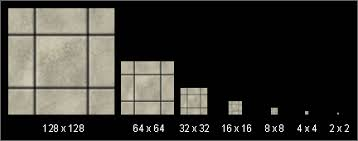
\includegraphics[scale=0.75]{Pictures/images.jpeg}
  \caption{Схематичне зображення MIP-текстурування}
  \label{fig:Mip}
\end{figure}

Зазвичай розміри текстур задані як степені двійки, наприклад, $$1024 \times 1024 = 2^{10} \times 2^{10}.$$ Це дозволяє легко створювати кожен наступний рівень MIP-текстури з деталізацією, зменшеною вдвічі порівняно з попереднім, тобто:
\[
\text{MIP}_{n+1} = \frac{\text{MIP}_n}{2}.
\]

Таким чином, кожен рівень зменшує площу текстури у чотири рази, а сумарне споживання пам’яті усіх рівнів MIP-текстур становить приблизно на $33\%$ більше, ніж для оригінальної текстури. Це випливає з геометричної прогресії площ:
\[
\sum_{n=1}^{\infty} \left(\frac{1}{4^n}\right) = \frac{1}{3}.
\]

Переваги використання MIP-текстурування полягають не лише в зменшенні навантаження на відеопам’ять та обчислювальні ресурси, але й у покращенні візуальної якості зображення. Зокрема, при рендерингу об’єктів, розташованих на значній відстані від камери, немає необхідності застосовувати пов\-но\-роз\-мір\-ну текстуру, адже спостерігач все одно не зможе розрізнити дрібні деталі. У таких випадках використовується менш детальна копія текстури, що знижує кількість вибірок у піксельному шейдері та підвищує продуктивність.

Окрім оптимізації, MIP-текстурування відіграє важливу роль у боротьбі з \textbf{муаровим ефектом}~(рис.~\ref{fig:Muar}) -- артефактом, що виникає внаслідок накладання високочастотної текстури на об’єкти, які займають невелику кількість пікселів на екрані. У таких випадках без MIP-текстурування може спостерігатися некоректна інтерполяція пікселів під час руху камери, що призводить до неприємного візуального мерехтіння.

\begin{figure}[h]
  \centering
  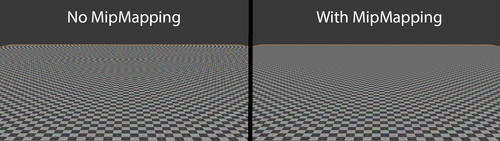
\includegraphics[scale=0.8]{Pictures/Mipmap_Aliasing_Comparison.png}
  \caption{Порівняння зображення з використанням та без використання MIP-текстурування}
  \label{fig:Muar}
\end{figure}
\newpage
\subsection{Рівень деталізації (Level of Detail, LOD)} \mbox{}\
\par Техніка рівня деталізації (LOD) полягає в динамічному виборі гео\-мет\-рич\-ної складності об'єкта залежно від відстані до камери. Ідея подібна до MIP-текстурування (рис.~\ref{fig:Mip}), але застосовується до геометрії (рис.~\ref{fig:LOD}), а не до текстур. У цьому підході для кожного об'єкта готується кілька версій моделі з різ\-ним числом полігонів -- від максимально деталізованої до значно спрощеної.

\begin{figure}[h]
  \centering
  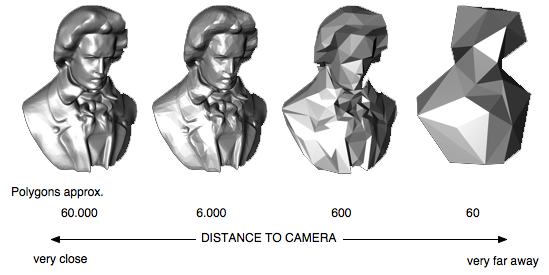
\includegraphics[scale=0.75]{Pictures/lod.png}
  \caption{Різні рівні деталізації}
  \label{fig:LOD}
\end{figure}

\par Під час рендерингу рушій або GPU автоматично вибирає відповідний рівень деталізації залежно від відстані до об'єкта чи його розміру на екрані. Наприклад, якщо об'єкт розташований далеко від камери, він займає менше пік\-се\-лів, і використання повністю деталізованої моделі стає недоцільним з точ\-ки зору продуктивності. Замість цього обирається менш складна геометрична версія, яка майже не відрізняється візуально на такій відстані, але значно знижує навантаження на GPU.

\par Подібно до MIP-текстурування, яке використовує різні версії текстури для зменшення артефактів та оптимізації пам’яті, LOD дозволяє досягти балансу між візуальною якістю та продуктивністю, зменшуючи кількість обчислень, необхідних для віддалених об’єктів. Це критично важливо у великих відкритих сценах, де на екрані одночасно може бути присутня велика кількість об’єктів.

\par У деяких випадках використовується так звана безперервна LOD (Con\-ti\-nuous LOD), де геометрія плавно змінюється замість різкого перемикання між рівнями, що дозволяє уникнути візуальних артефактів у вигляді ``помітного стрибка`` при зміні моделі.

\subsection{Відкладене освітлення та затінювання (Deferred Shading)} \mbox{}\
\par Однією з найефективніших технік оптимізації рендерингу в сучасних графічних рушіях є відкладене освітлення та затінювання (Deferred Shading). Ос\-нов\-на ідея полягає в розділенні етапів рендерингу сцени на дві фази: збір геометричної інформації та обрахунок освітлення.

\par На першому етапі виконується рендеринг геометрії сцени у так звані G-буфери (geometry buffers) (рис.\ref{fig:G}) -- набір текстур, що зберігають усю необхідну інформацію про пікселі:
\begin{itemize}
\item глибину (depth buffer, z-buffer);
\item нормалі поверхонь (normal buffer);
\item базовий колір (albedo);
\item властивості матеріалів, такі як шорсткість і металічність (roughness-metalness buffer).
\end{itemize}

\begin{figure}[h]
  \centering
  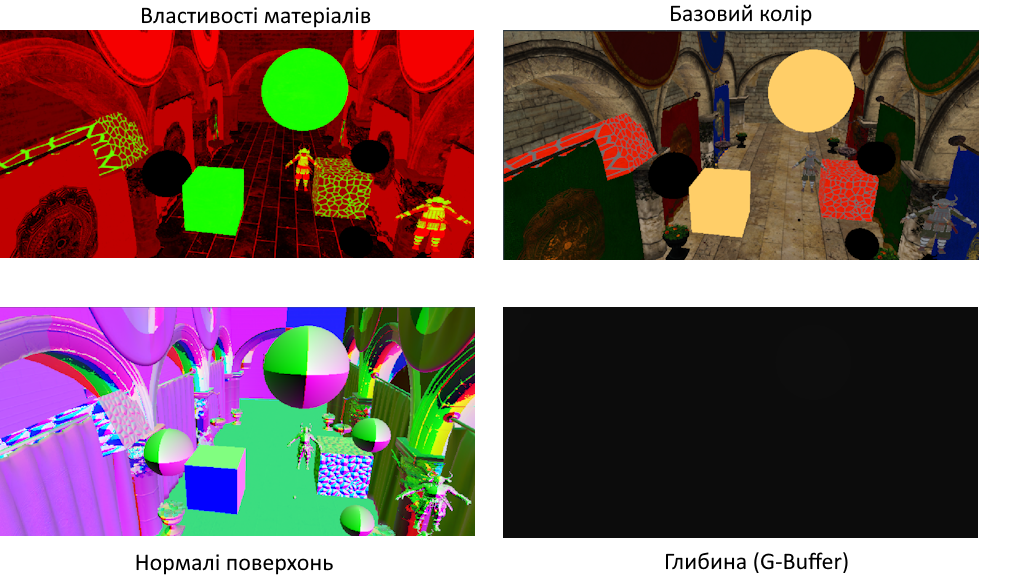
\includegraphics[scale=0.75]{Pictures/G-buffer.png}
  \caption{G-буфери}
  \label{fig:G}
\end{figure}


\par Після цього, на другому етапі, система виконує обчислення освітлення, використовуючи інформацію з G-буферів лише для пікселів, що дійсно потрапили у фінальний кадр. Таким чином, обчислення освітлення відбувається лише для видимих фрагментів, що значно зменшує кількість непотрібних операцій порівняно з прямим (forward) рендерингом, де освітлення розраховується для всіх об'єктів незалежно від того, чи видно їх на екрані.

\par Основною перевагою відкладеного затінювання є його масштабованість при великій кількості джерел світла, оскільки світло розраховується по\-ст\-фак\-тум у екранізованому просторі, а не для кожного пікселя кожного об’єкта окремо. Це дозволяє значно підвищити продуктивність у складних сценах із ба\-гать\-ма джерелами світла.

\par Водночас, варто враховувати і недоліки: зокрема, складність підтримки прозорих об’єктів, високі вимоги до пам’яті GPU через велику кількість G-буферів, а також обмеження при використанні MSAA (Multisample Anti-Alia\-sing).

\section{Результати числових експериментів}

\par У цьому підрозділі наведено результати реалізації основних теоретичних положень, розглянутих у попередніх розділах, зокрема методів фізично коректного рендерингу (PBR), мік\-ро\-фа\-сет\-ко\-вої BRDF-моделі Кука–Торренса, процедур MIP-мапінгу, організації рівнів деталізації, реалізації відкладеного затінення (deferred shading), а також оптимізаційних технік, що були інтегровані у рендеринг-пайплайн.

\par Перш ніж перейти до поетапного аналізу впливу окремих фізичних параметрів на результуюче зображення, на рис.~\ref{fig:overview} та \ref{fig:close_overview} продемонстровано загальний вигляд сцени, що візуалізує повноцінну реалізацію системи освітлення із урахуванням усіх складових PBR-моделі.

\begin{figure}[h]
\centering
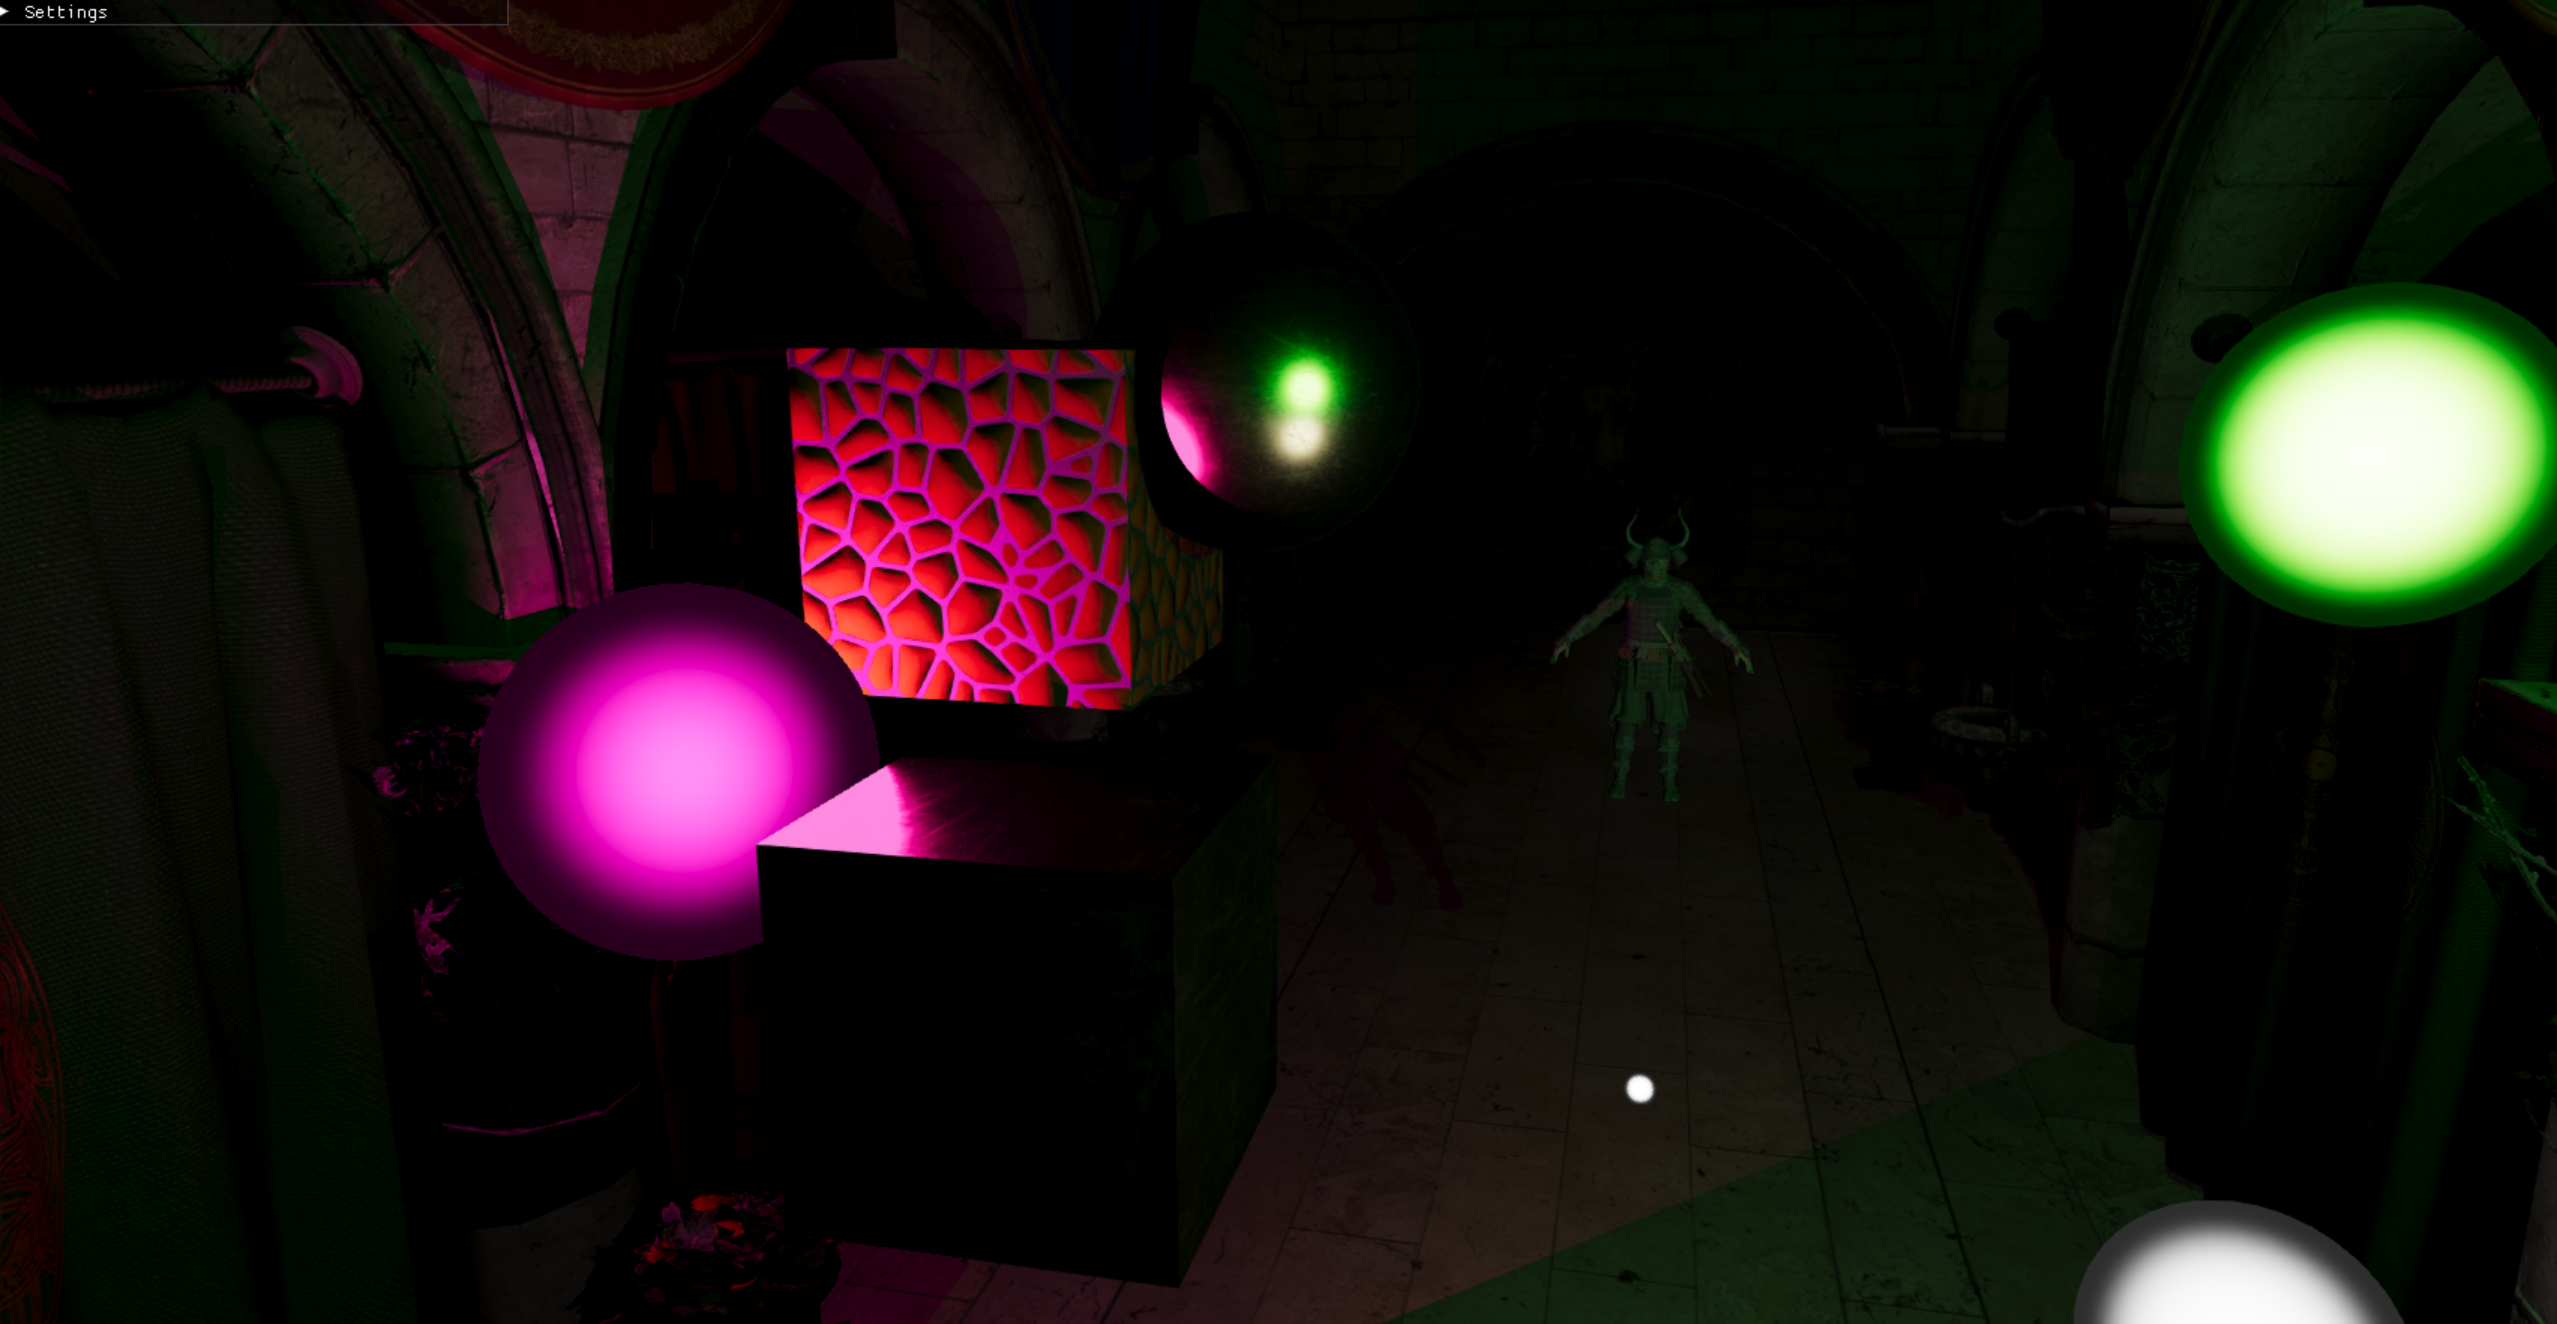
\includegraphics[scale = 0.2125]{Pictures/1.png}
\caption{Загальний вигляд сцени з реалізованою PBR-системою}
\label{fig:overview}
\end{figure}

\begin{figure}[h]
\centering
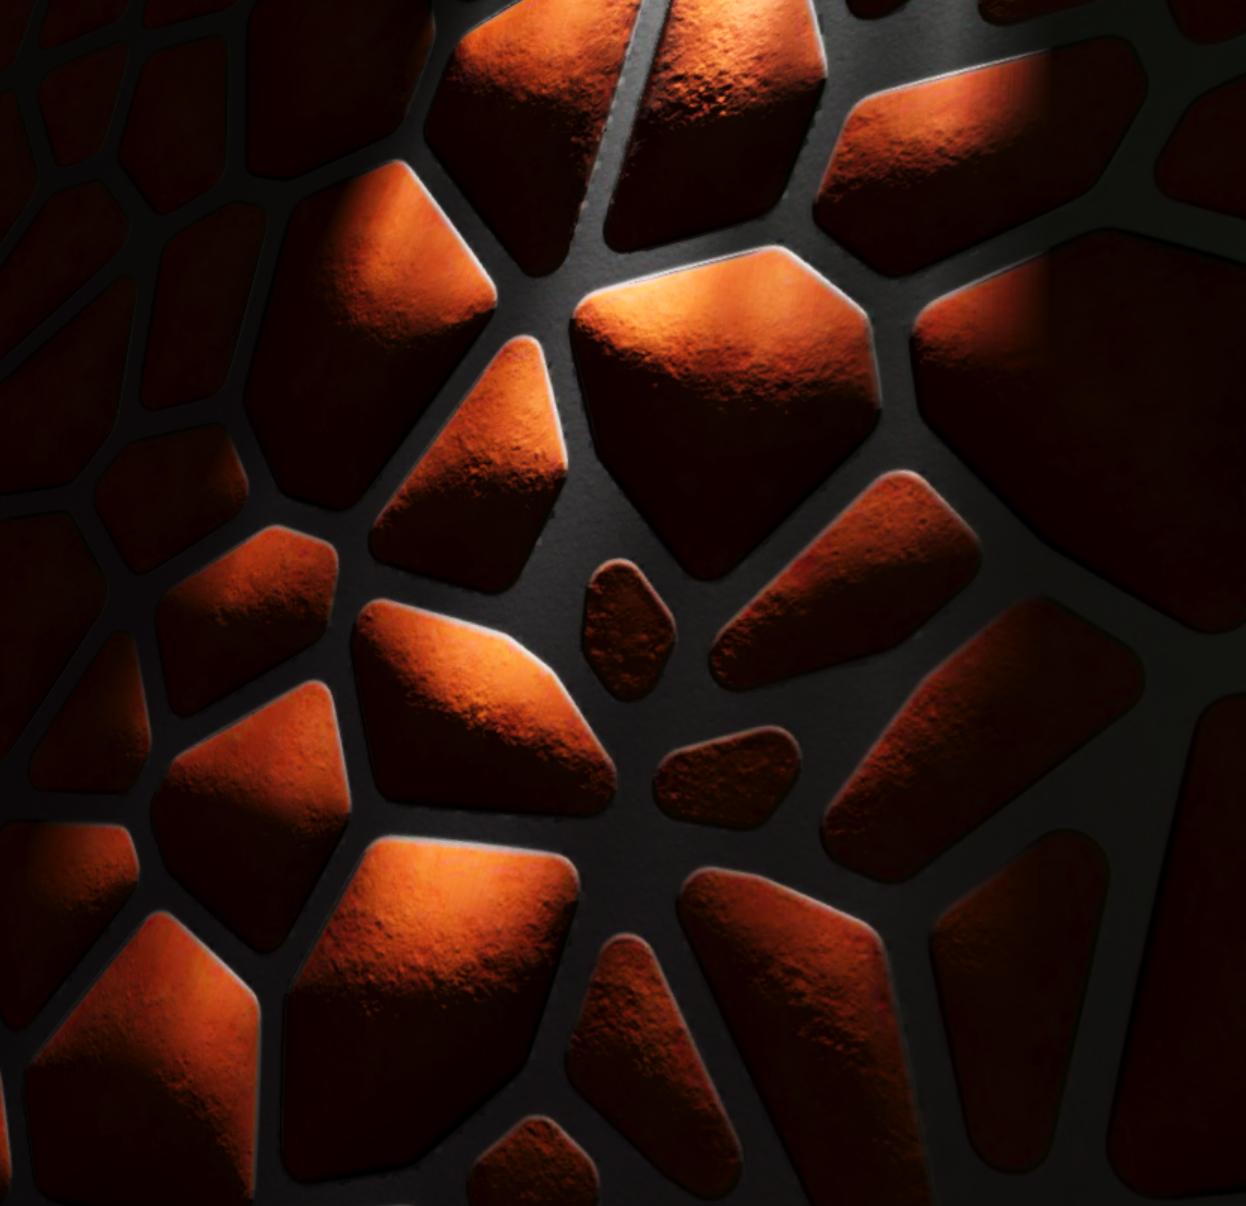
\includegraphics[scale = 0.2125]{Pictures/12.png}
\caption{Фрагмент сцени: вигляд об'єктів крупним планом}
\label{fig:close_overview}
\end{figure}

\par Для демонстрації впливу матеріальних властивостей на вигляд поверхні було проведено серію експериментів із візуалізацією сферичних об’єктів при різних значеннях параметрів металічності ($metalness$) та шорст\-кос\-ті ($roughness$). Зокрема:

\begin{itemize}
\item Металева сфера з $metalness = 1.0$ та $roughness = 0.5$, з просторовими варіаціями параметрів по поверхні -- демонструє роботу мікро\-фа\-сет\-ко\-вої BRDF-моделі.
\item Та ж сфера з високою шорсткістю ($roughness = 0.9$), що зумовлює розмиття дзеркального відбиття.
\item Ідеально гладка металева сфера ($roughness = 0.0$), яка відображає навколишнє середовище з максимальною чіткістю.
\item Діелектрична сфера ($metalness = 0.0$), яка не створює дзеркального відбиття, натомість формує лише дифузне розсіювання світла.
\end{itemize}

\begin{figure}[h]
\centering
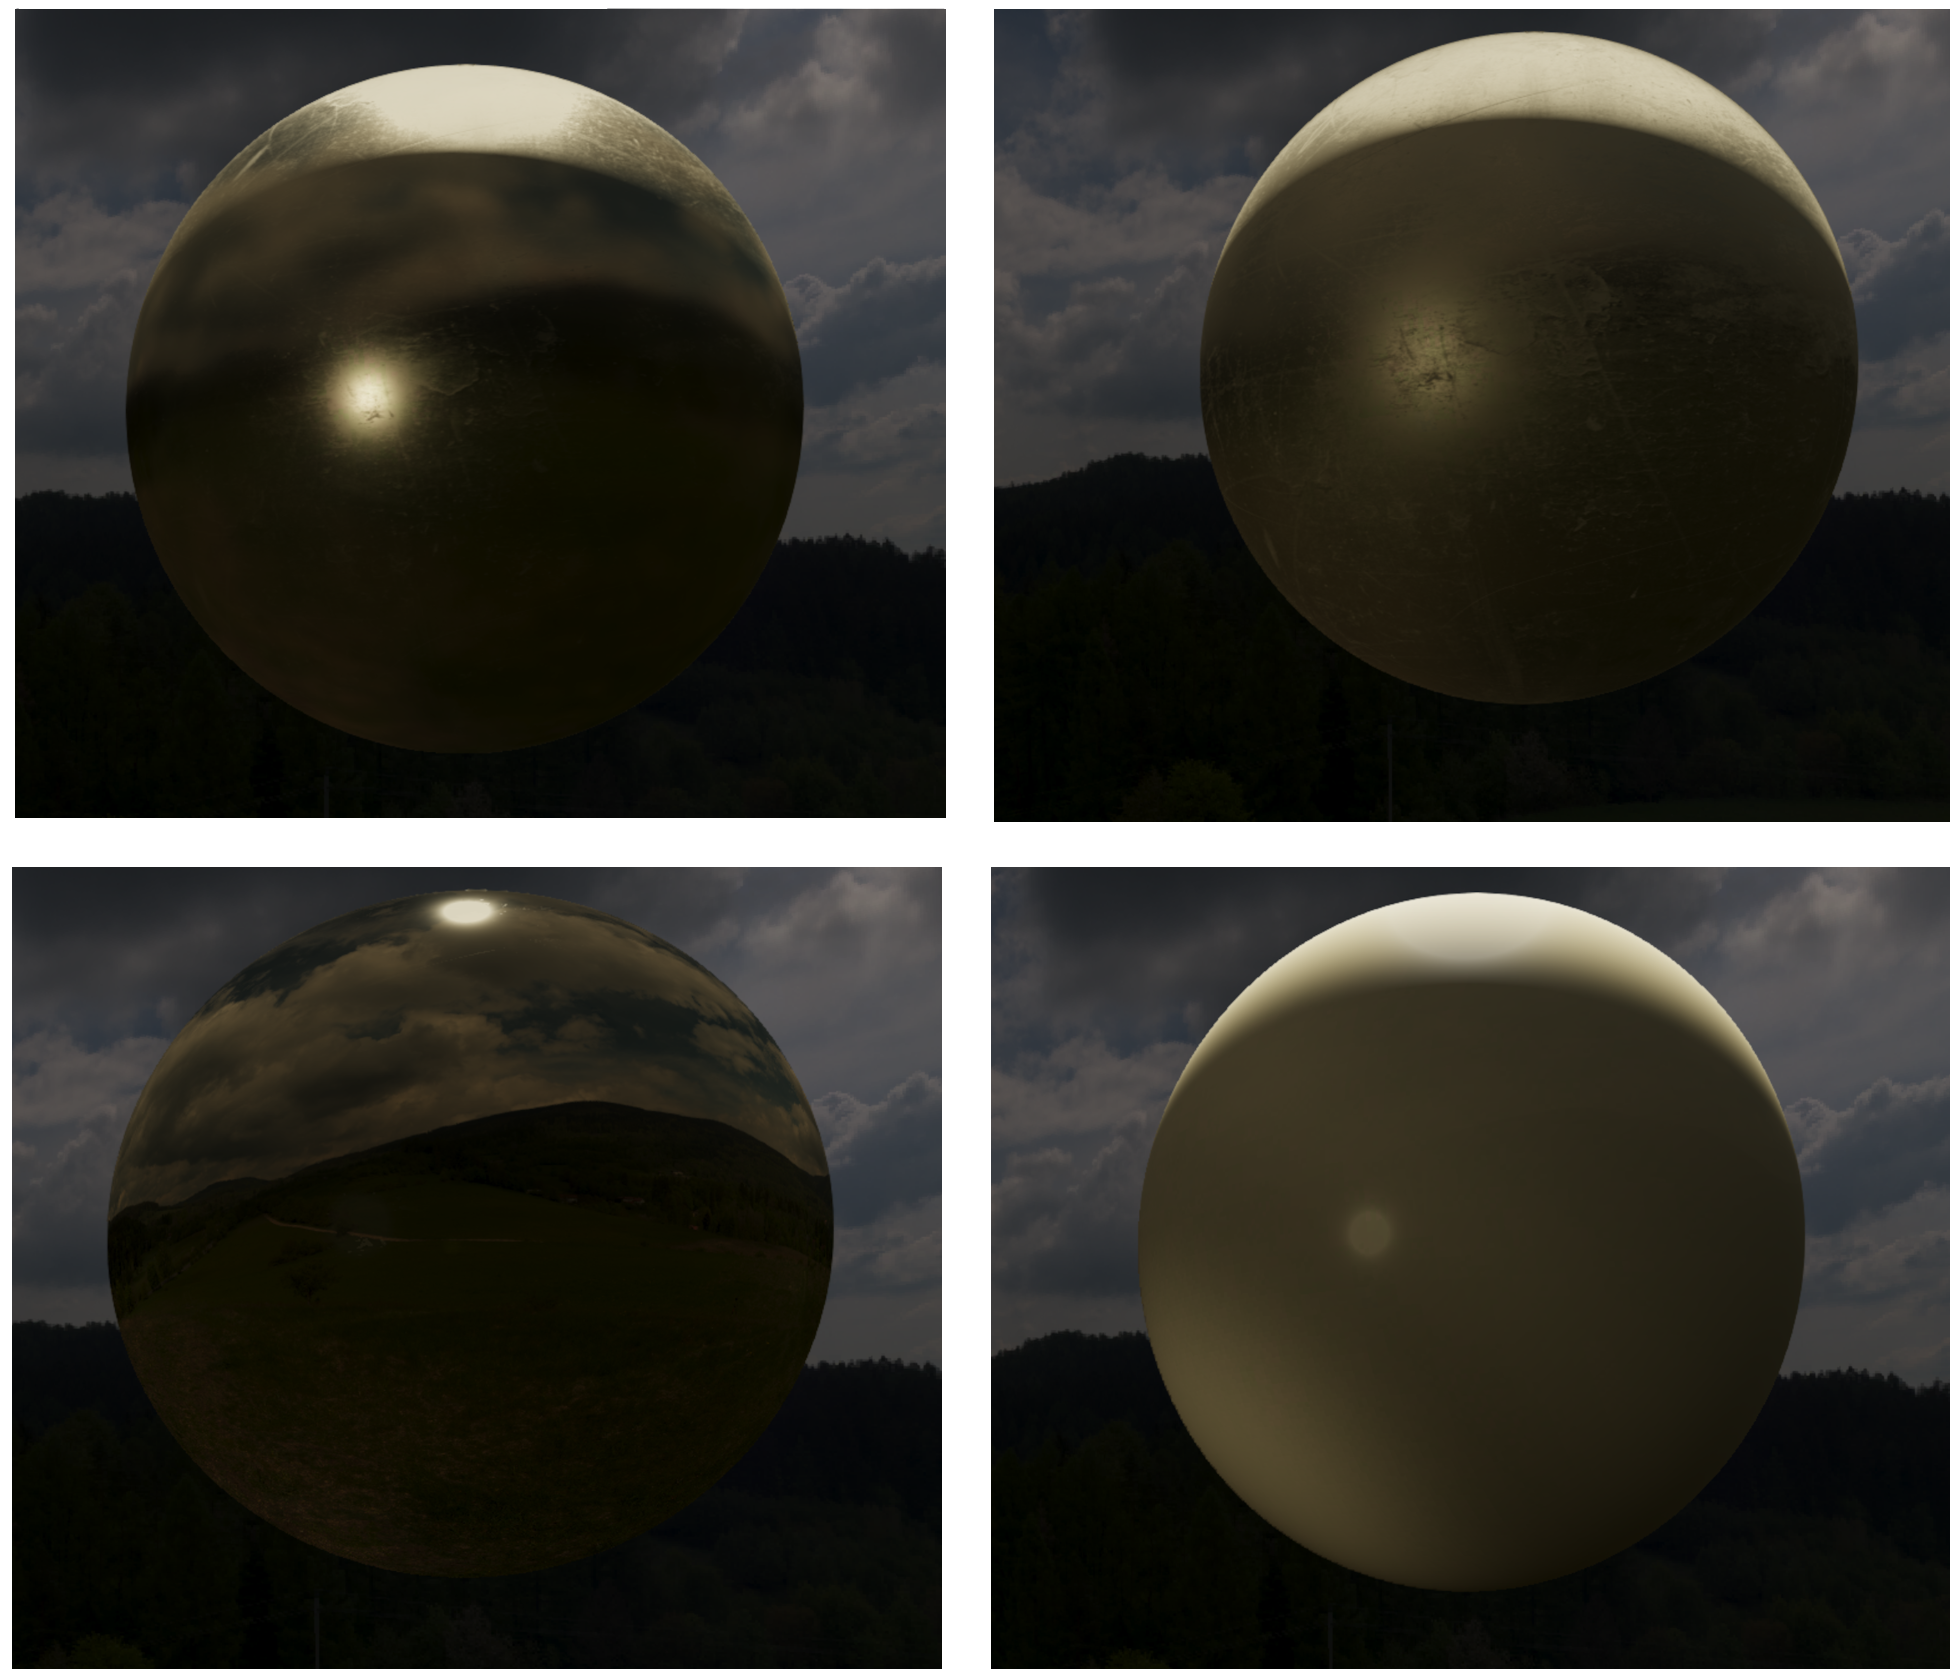
\includegraphics[width=0.8\linewidth]{Pictures/SphereComparance.png}
\caption{Порівняння вигляду сфер з різними фізичними параметрами}
\label{fig:sphere_comparison}
\end{figure}

\par Як видно з результатів, металева сфера відображає навколишнє середовище, причому ступінь розмиття відбиття прямо залежить від значення шорст\-кос\-ті: чим вище $roughness$, тим дифузнішим і менш чітким стає дзеркальне відбиття. У випадку діелектричної сфери відображення довкілля практично відсутнє; поверхня переважно демонструє дифузне розсіювання світла без характерного блиску, що відповідає фізичній поведінці неметалевих матеріалів.

\par Наступним етапом є візуалізація складнішого тривимірного об’єкта — моделі самурая (рис.~\ref{fig:samurai_full}). Зображення наведено поетапно, із поступовим відключенням окремих складових освітлення, з метою наочної демонстрації їх внеску у фінальне зображення:

\begin{enumerate}
\item Повна модель з активованими всіма компонентами освітлення (diffuse + specular).
\item Лише дифузна складова — демонструє розсіювання світла поверхнею.
\item Лише дзеркальна (specular) складова — ілюструє відбиття світла відповідно до мікрофасеткової моделі.
\end{enumerate}

\begin{figure}[h]
\centering
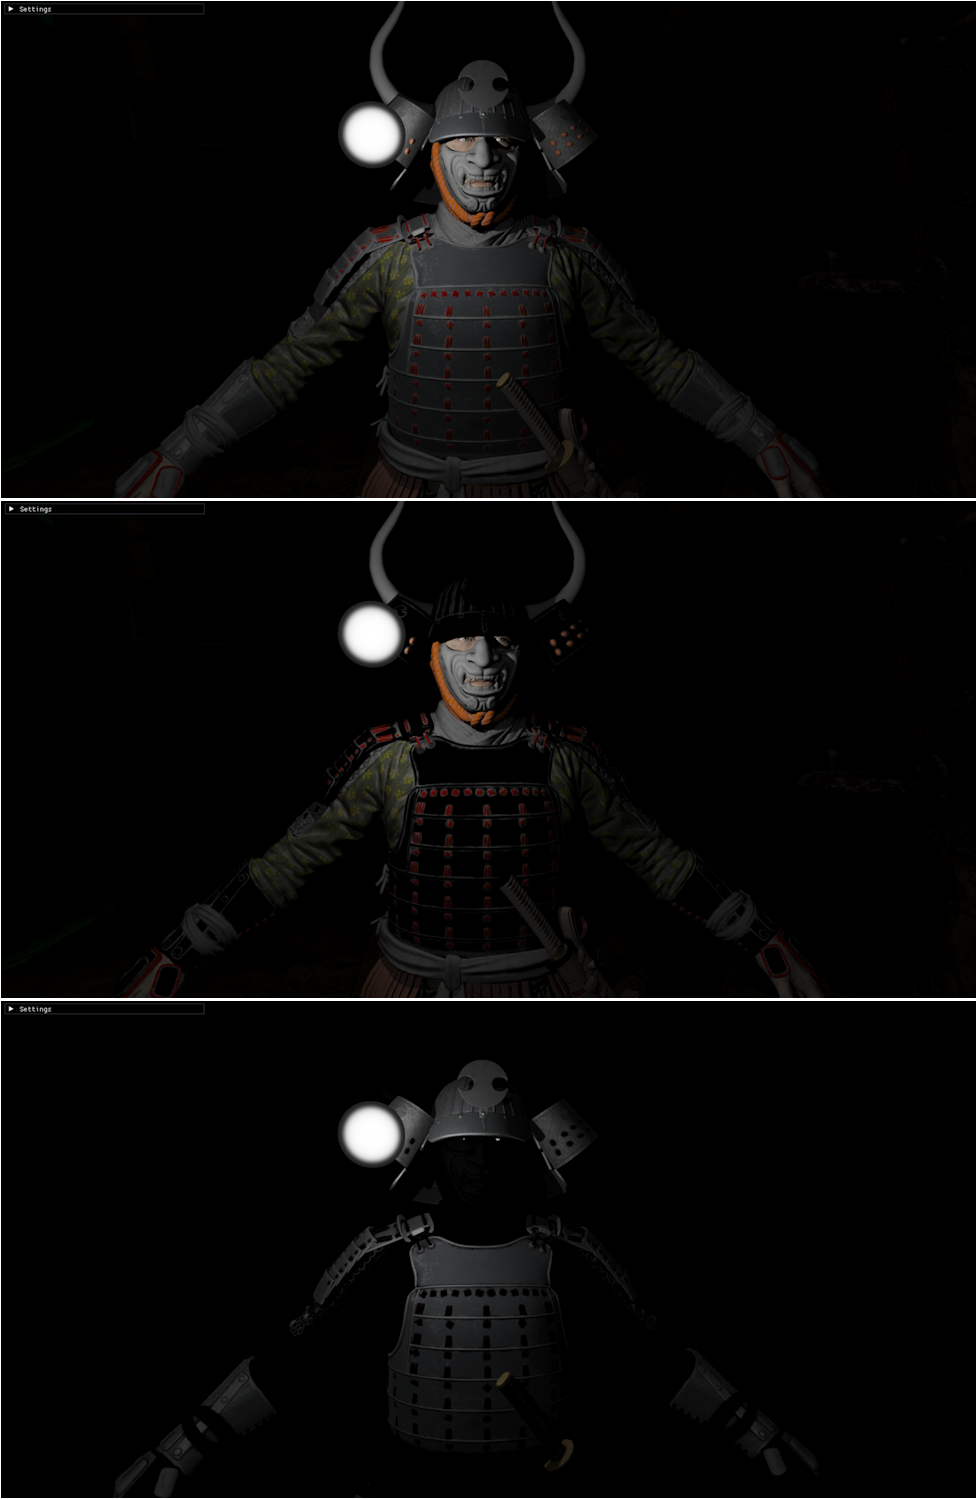
\includegraphics[scale=0.35]{Pictures/Samuraifull.png}
\caption{Порівняння вигляду моделі самурая при різних конфігураціях освіт\-лен\-ня}
\label{fig:samurai_full}
\end{figure}

\par Як видно з результатів (рис. \ref{fig:samurai_full}), при візуалізації лише дифузної складової металічні поверхні втрачають колір та виглядають тьмяно. Це пояснюється тим, що згідно з фізичними властивостями металів, дифузна складова майже повністю відсутня -- більшість світла або поглинається, або дзеркально відбивається. Навпаки, при візуалізації лише дзеркальної складової поверхні ді\-елект\-ри\-ків виглядають майже повністю темними, оскільки для них дзеркальна компонента є дуже слабкою.

\par Таким чином, проведені числові експерименти підтверджують коректність реалізованої моделі фізично обґрунтованого освітлення та її відповідність очікуваній фізичній поведінці матеріалів при різних параметрах. Отримані результати демонструють узгодженість моделі з фундаментальними законами оптики, зокрема законом збереження енергії, ефекту Френеля та властивостями мікрофасеткових відбиттів, що проявляється у правильному відтворенні таких явищ, як розмиття дзеркальних рефлексій при збільшенні шорсткості, слабке відбиття у діелектриків та кольорове віддзеркалення у металів. Це вказує на адекватність математичного апарату, використаного при дискретизації рівняння рендерингу та BRDF-моделі, а також підтверджує ефективність програмної реалізації в умовах складних сцен. Крім того, результати ілюструють високу якість візуалізації, яка досягається за рахунок правильного врахування геометричних, спектральних та освітлювальних параметрів при моделюванні.
